\documentclass[11pt]{scrartcl}

\usepackage{pgf, tikz}
\usetikzlibrary{arrows, calc}

\newcommand{\drawPentagon}{
    \def\len{5cm}
    \coordinate (O) at (0,0);
    \coordinate (P0) at (0:\len);
    \coordinate (P1) at (70:\len);
    \coordinate (P2) at (140:\len);
    \coordinate (P3) at (210:\len);
    \coordinate (P4) at (280:\len);
    \coordinate (P5) at (350:\len);

    \foreach \i in {0,1,2,3,4,5}{
        \draw (O) -- (P\i);
    }

    \draw (P0) -- (P1) -- (P2) -- (P3) -- (P4) -- (P5);

    \node[rotate=15] at (barycentric cs:O=1,P1=1,P2=1) {GAP Days Fall 2017};
    \node[rotate=155] at (barycentric cs:O=1,P3=1,P4=1) {Simplicial Surfaces};
}

\usepackage[absolute]{textpos} 	% Absolute Textposition ermöglichen

\begin{document}
	\pagenumbering{gobble}
	\begin{textblock}{3}(-0.1,0.1)
            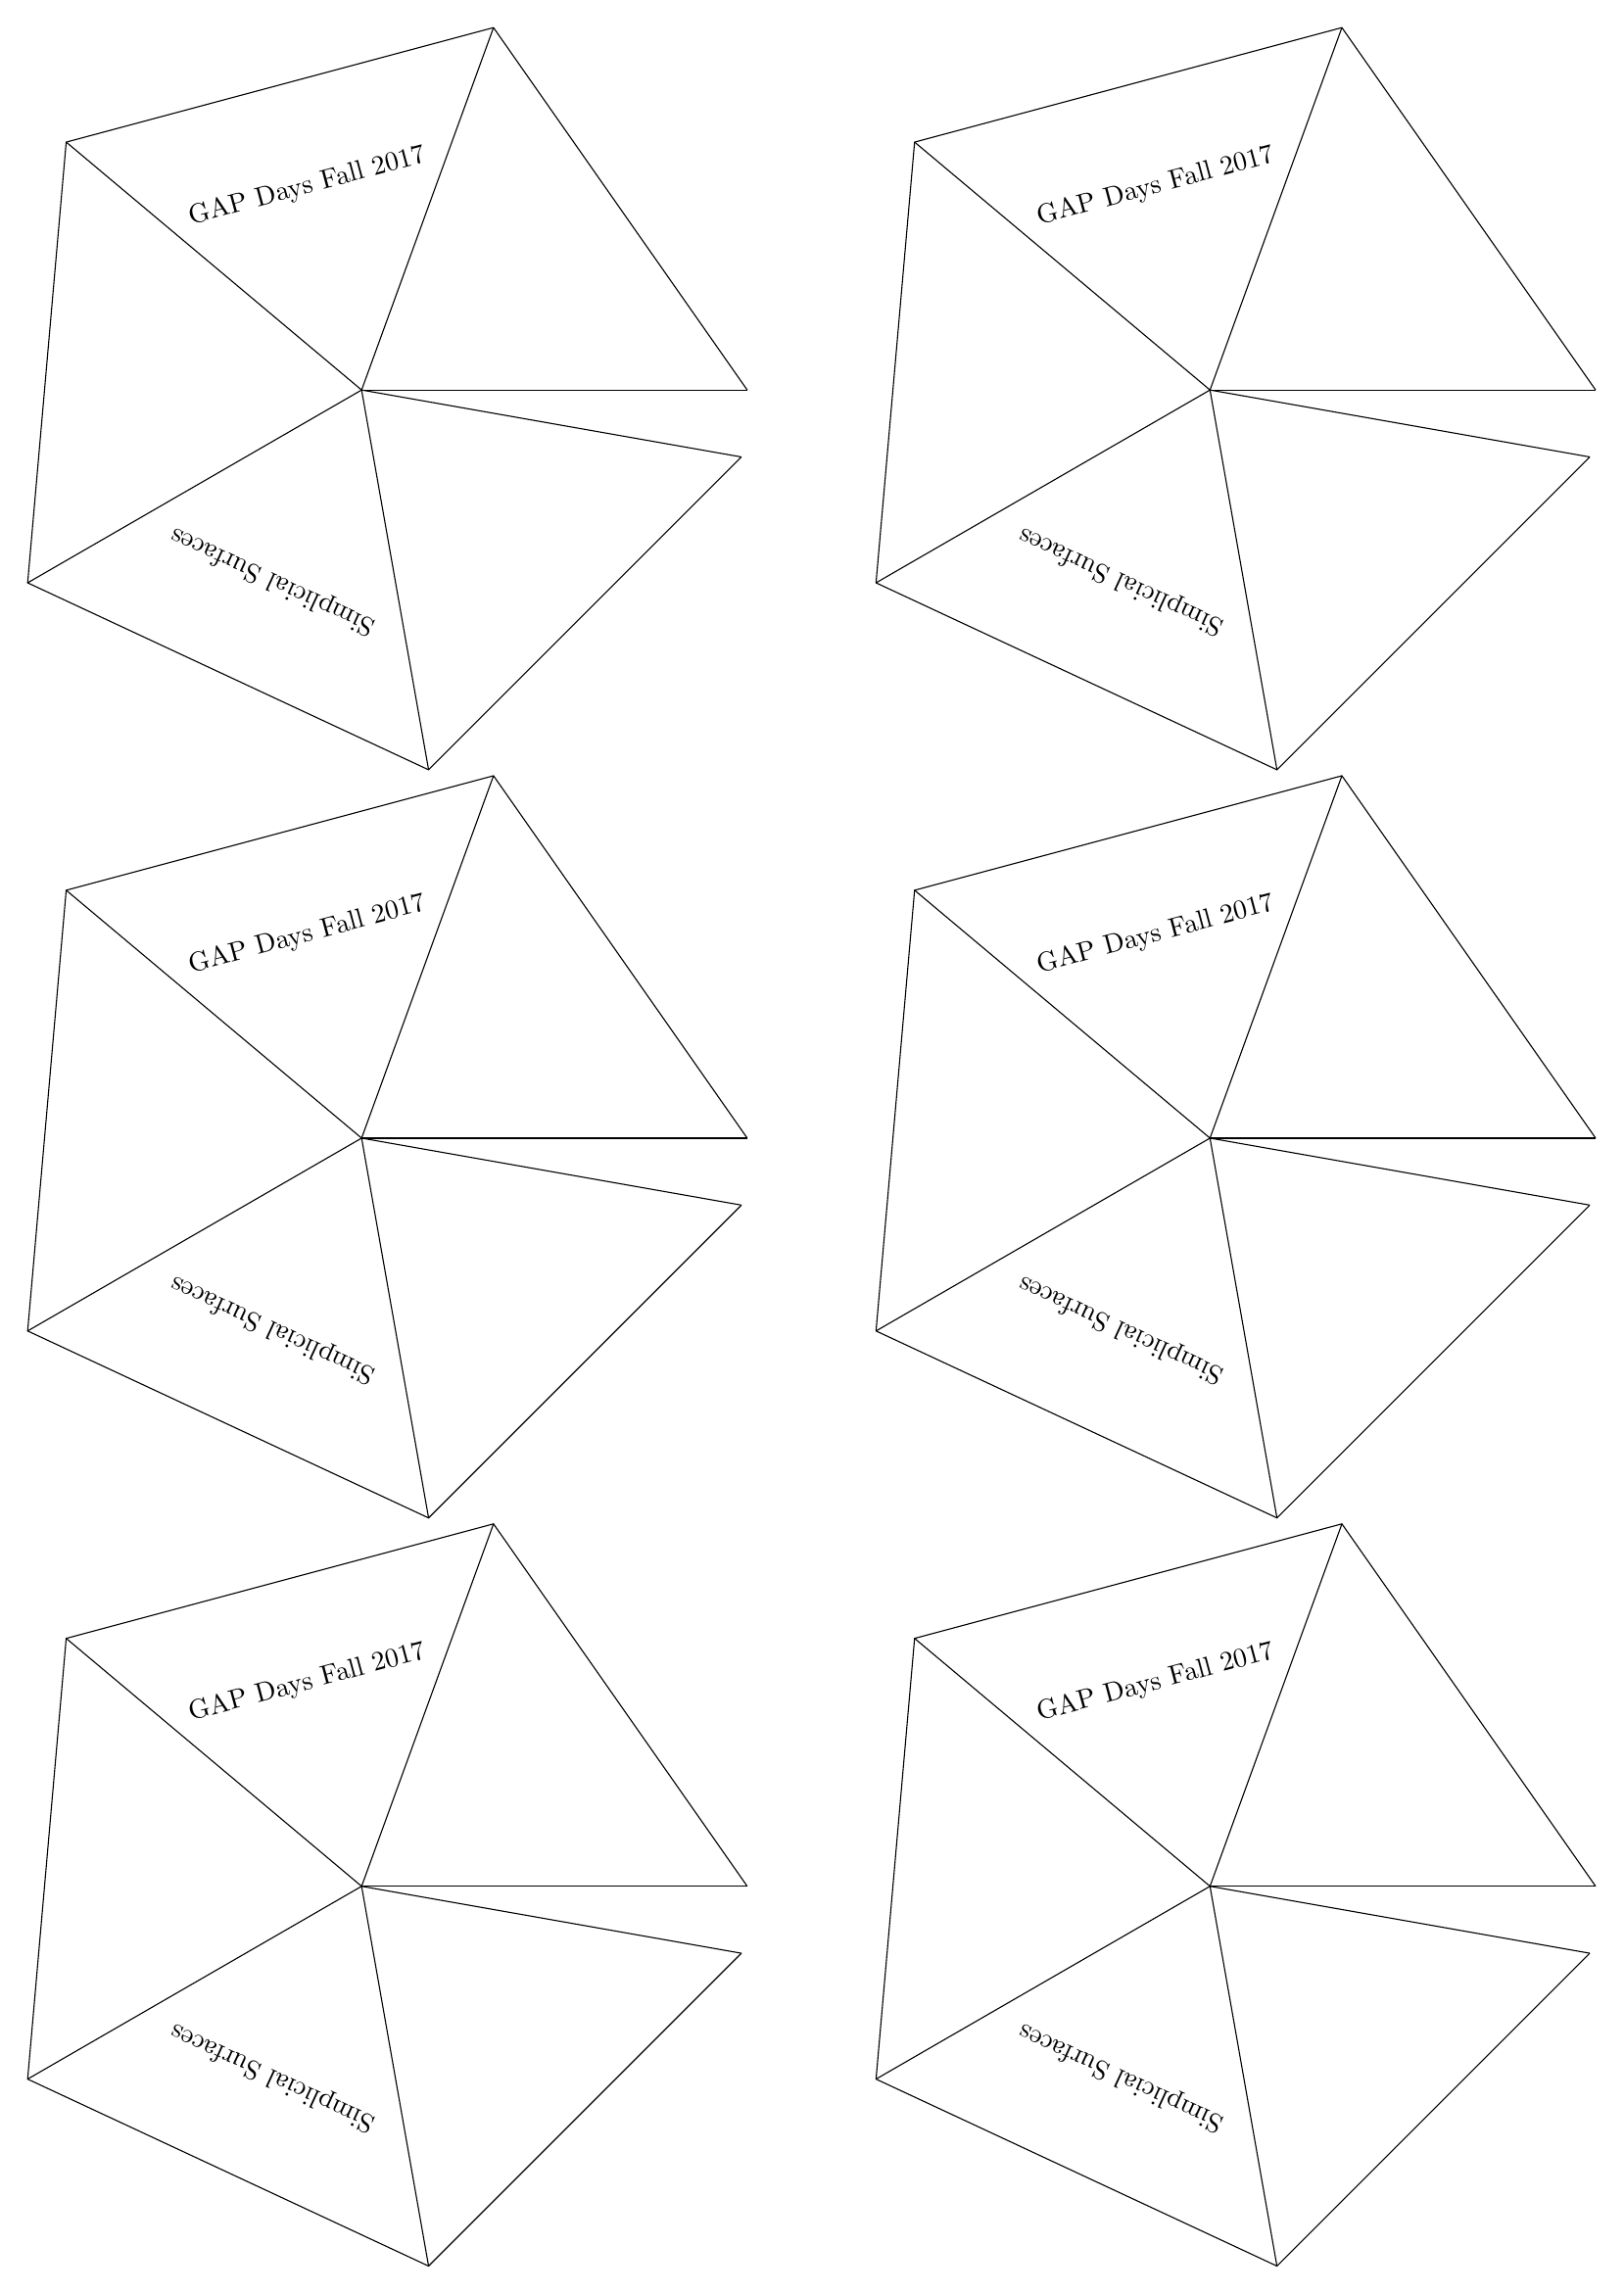
\begin{tikzpicture}
                \def\XA{3cm}
                \def\XB{14cm}
                \def\YA{3cm}
                \def\YB{12.7cm}
                \def\YC{22.4cm}
                \begin{scope}[xshift=\XA,yshift=\YA]
                    \drawPentagon
                \end{scope}

                \begin{scope}[xshift=\XB,yshift=\YA]
                    \drawPentagon
                \end{scope}

                \begin{scope}[xshift=\XA,yshift=\YB]
                    \drawPentagon
                \end{scope}

                \begin{scope}[xshift=\XB,yshift=\YB]
                    \drawPentagon
                \end{scope}

                \begin{scope}[xshift=\XA,yshift=\YC]
                    \drawPentagon
                \end{scope}

                \begin{scope}[xshift=\XB,yshift=\YC]
                    \drawPentagon
                \end{scope}
            \end{tikzpicture}
	\end{textblock}
\end{document}
